\chapter{Design}
\label{chapter:Design}
%Overarching design in a top-down view: 
%-server/client design overall architecture, system model
%-describe file system, 
%-how protocol is peformed by the server
%-describe current functionality of the implementation. Handles protocol run, view-changes and checkpointing

%old version:-overall usage over different parameters, overaching stuff thats not the actual implementation of the algorithm, but the network layer to server to algorithm, how to run the algorithm/checkpointing/view changes.
%first draft!!!
%This chapter present an overall summary of the PBFT application implemented. This includes a brief summary of the system model used for performing the PBFT algorithm. The structure of the application including a brief introduction to its file structure as well as describing the general design for performing the consensus algorithm. We will finally describe the current functionalities that are present in the current application. 
This chapter presents an overall summary of our PBFT application implementation. This includes a description of the system model used for the PBFT network. Additionally, to better understand the workflow of the application, a summary of the file structure used is given. Finally, a description is provided for the current application design. Primarily specifying the which parts of the program take advantage of the Cleipnir framework and how the server side interacts with the protocol workflow.
%Remember to check previous sections for how I should mark names in the text!
\section{System Model}
\begin{figure}
	\centering
	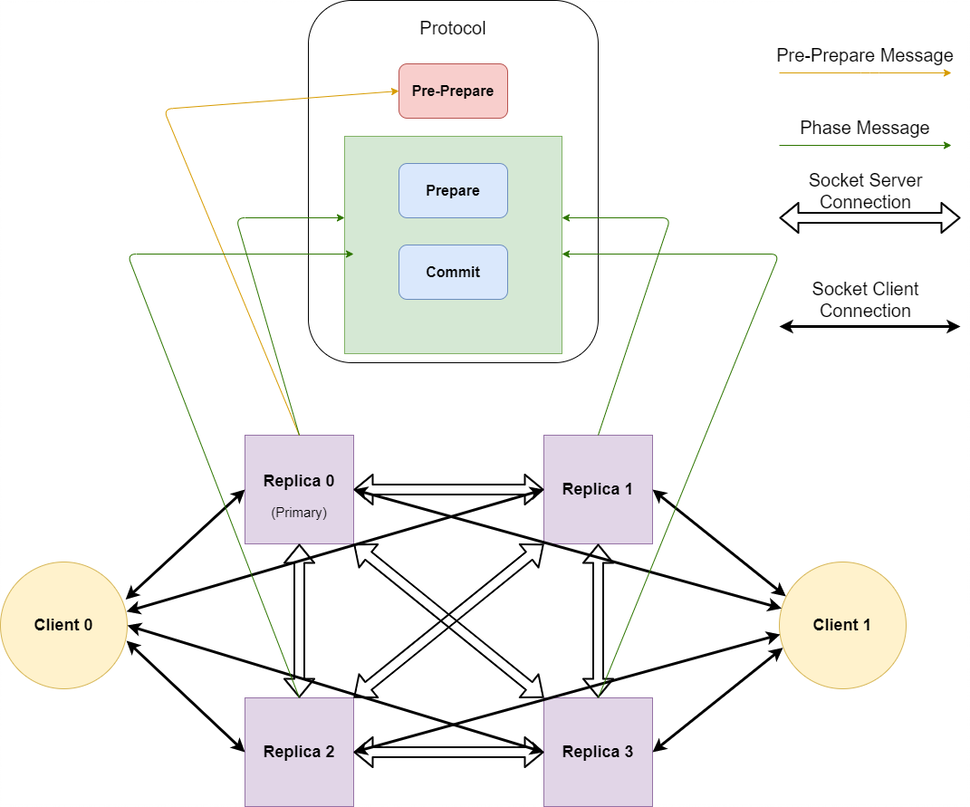
\includegraphics[width=\linewidth]{figures/meshnetwork}
	\caption{Overall architecture of the PBFT implementation networking}
	\label{fig:meshnetwork}
\end{figure}
The \autoref{fig:meshnetwork} shows the system model used for PBFT implementation. Generally our system model follows the same structure as the system model introduced in \autoref{sec:systemModel}. The system consists of four server implementations called \emph{replicas}, where the replica with the lowest identifier value is chosen as the primary. These four replicas are communicating over a mesh network using socket connections. This means each replica shares a unique network socket with each other replica in the PBFT network. To avoid creating multiple socket connections between two replicas, the replica with the highest identifier is the one tasked with being the initiator when creating the socket connection. Because of this the primary replica is not required to be active party when establish any connections to its fellow replicas. The primary instead establishes all its socket connections by listening for any connections attempts on its local network address. The opposite scenario occurs for the replica with the highest identifier value. Although the replica still listens for connections on its local network address in the case where a higher replica does exist in the network, it is also responsible for initiating the socket connections with all the other replicas in the network that has lower identifier values to its own.

When the replicas have established connections, the replicas can still not fully communicate with each other until they have exchanged public keys. This is required so that messages between replicas can be verified using a digital signature. Public keys are exchanged in \emph{session messages}, which are messages that are automatically sent between replicas once a socket connection has been established. If the public keys are for some reason not exchanged, then the replica discards any message received from that host. If the message received from the unknown host happens to be a \emph{request} or a \emph{phase message}, the replica also terminates the connection. This also applies for clients. This current public key model is unfortunately not very secure. This is due to public keys being ephemeral, therefore it needs to be updated and replaced in the case the replica’s execution is interrupted or stopped. Currently in this implementation, the private and public key pair for a replica are randomly created at system start-up. Since currently there is no way for the replicas to authenticate another replica after it has rebooted. A replica must replace the key value pair representing a replicas public key in its register if it receives a new session message with the same replica identifier value. This in turn means the system is susceptible to impersonation and spoofing attacks~\cite{ WEB:spoofingAttack}. Because the main goal of this thesis focuses more on the aspects behind implementing a simple PBFT workflow, the current cryptographic system was deemed sufficient for simulating a network using digital signatures. However, it is important to be aware of this major security flaw of system so that it can be potentially fix it in the future. Not to mention avoid similar problems in the future.

The system performs the PBFT protocol by exchanging protocol messages over the mesh network until atleast three of the servers have finished all three protocol phases. In this implementation protocol messages are referred to as \emph{phase messages}. The PBFT protocol is trigger when the server receives a request from one of the connected client nodes. The primary is responsible for officially starting an instance of the PBFT protocol by multicasting a phase message of type pre-prepare. There are two important goals for the pre-prepare phase. The first is to make sure that the replicas have an agreement upon the ordering of the request. In other words, the replicas will perform the requests in the same order as the primary, which in turn means the request should have the same sequence numbers throughout the network. The second important goal is to determine whether or not the primary is fit to be leader. As mention in section \autoref{sec:view-change}, a view-change occurs when a leader no longer is eligible. In our application the view-changes are triggered by timeout which are set once a replica receives a client's request. If the primary takes too long in the pre-prepare phase, than the timeout will exceed and the other replicas will perform a view-change in order to change the primary replica. Although it would be useful to have timeouts in the commit phase in the instance where majority of servers are unable to properly finish the commit phase, it is currently not supported in our implementation due to how timeouts are handled inside the protocol workflow(should probably be moved elsewhere). The rest of the replicas will be the responsible party during the prepare phase by sending phase messages of type prepare, while every replica will participate in the commit phase using commit type phase messages. The last step of current PBFT implementation is to create a reply message and send it back to client responsible for the request. The details in regards to the PBFT workflow implementation will be discussed in \autoref{chapter:Imp}.

\section{File structure}
In figure we \autoref{fig:filestruct} can see a short summary of the file system for our PBFT replica. The summary shows the root folders in our PBFT replica implementation. The summary also highlight some of the more important files, meaning files containing the most relevant code segments. 

\subsection{Folders}
To start of the PBFT implementations uses a lot of different types of message objects which are defined in their own seperate file. Therefore, all of the different message classes are stored within the \emph{Messages} folder. This includes interface that are shared among messages types. Similarly, there are several objects known as certificates which are used within this PBFT implementation and its class files and interfaces are stored within the \emph{Certificate folder}. Certificates are essentially records showing the status for the protocol states. For instance, the replica has a log which stores two certificates for each requests successfully handled by the PBFT protocol. These two certificates in the log will acts as proof for successful prepare and commit phases for that specific sequence number. 

The \emph{Helper} folder contains all the static functions used in the PBFT implementation that are not linked to any specific object instance. This includes functionality for serializing and deserializing messages objects with JSON~\cite{WEB:NewJSON}, cryptographic functions related to creating and validating digital signatures and files containing all the enum types used for this thesis. An enum is essentially a predefined dotnet class that has only constant values which are defined upon initialization and is really useful for classifying other objects~\cite{WEB:Enum}. In our PBFT implementation we have for instance used enums to categories the protocol phase a phase message belongs to. This allows the program to easily distinguish between pre-prepare, prepare and commit phase messages.  

The \emph{JSONFiles} contains the JSON files which contains the network addresses for each of the replicas in the system designated to their receptive identifier values. There exist two JSON files in this folder. The first file is used when running the implementation over multiple systems or over docker containers. The second file uses localhost addresses with different port numbers at is meant to be used when testing the system on a local device.

The PBFT replica implementation uses Cleipnir to persist important parts of the code in order for servers to easily be able to reconnect to the system. As discussed in \autoref{chapter:Cleipnir}, Cleipnir has several different engine types which can be used to serialize and store the applications data. In our PBFT replica implementation, we have decided to use the \emph{Simple File Storage} engine. The \emph{Storage} folder will contain the .txt files in which Cleipnir stores its data in. Since there are several instances of replicas in the PBFT network, the name of the .txt file used to store the application data will follow the structure "PBFTStorage" with the replicas identifier value at the end of the name.

The \emph{Replica} folder contains code which are directly related to the server or code which are directly related to the protocol. The \emph{Replica} folder has two sub folders in order to easier distinguish between the files. The subfolder \emph{Network} contains code related to networking part. This includes the creation of sockets and functions for properly handling the data received from the socket by the TCP network protocol. 
The \emph{Protocol} sub folder contains code which are directly related to the protocol execution. This folder contains code related to the main workflow of the PBFT algorithm. In addition, code for handling the reactive execution for view-change and checkpointing can also be found in this folder.
The other files in the \emph{Replica} folder contains code that helps the replica run properly, including code which are used to help communication between server side and protocol workflow run inside Cleipnir.
The \emph{Storage} 

\subsection{Files}
The \emph{App.cs} file contains the code which starts all the processes needed in the PBFT replica. This includes code for starting Cleipnir, creating a server instance and starting the protocol handlers. This file also includes the main application state, which in this implementation is simply a list of operations theoretically performed by the system.

The \emph{Server.cs} file is by far the largest. This is due to the \emph{Server.cs} file being the bridge linking the network layer, responsible for sending and receiving messages properly, to the active protocol which requires the result of said messages. In addition to in general being responsible for most of the replica server side operations. 

The \emph{Workflow.cs} file is where the code for normal protocol workflow is stored, as well as where the code for performing the view-change protocol is stored. We will introduce the workflow found in this file in \autoref{chapter:Imp}
%\newpage
\begin{wrapfigure}{r}{0.45\linewidth}
\centering
%\vspace{15pt}
%\rule{0.9\linewidth}{0.75\linewidth}
% ,scale=0.8, every node/.style={scale=0.8}
\tikzstyle{every node}=[draw=black,thick,anchor=west]
    \begin{tikzpicture}[%
      grow via three points={one child at (0.5,-0.7) and
      two children at (0.5,-0.7) and (0.5,-1.4)},
      edge from parent path={(\tikzparentnode.south) |- (\tikzchildnode.west)}]
      \node {PBFT}
        child { node {App.cs}}
        child { node {Certificates}
        	child {node {...}}
        	}	
        child [missing] {}
        child { node {Messages}
        	child {node {...}}
        	}
        child [missing] {}
        child { node {Helper}
        	child {node {...}}
        	}
        child [missing] {}
        child { node {JSONFiles}
        	child {node {serverInfo.json}}
        	child {node {testServerInfo.json}}
        	}
        child [missing] {}
        child [missing] {}
        child { node {Storage}
        	child {node {...}}
        }
        child [missing] {}
        child { node {Replica}
          child { node {Server.cs}}
          child { node {Network}
          	child {node {...}}
        	}
        }
        child [missing] {
          child { node {Protocol}
          child { node {Workflow.cs}}
          child { node {...}}
        	}
        };
\end{tikzpicture}
    \caption{Summary of the file architecture for the PBFT implementation}
    \label{fig:filestruct}
    \vspace{40pt}
\end{wrapfigure}

\begin{figure}[H]
	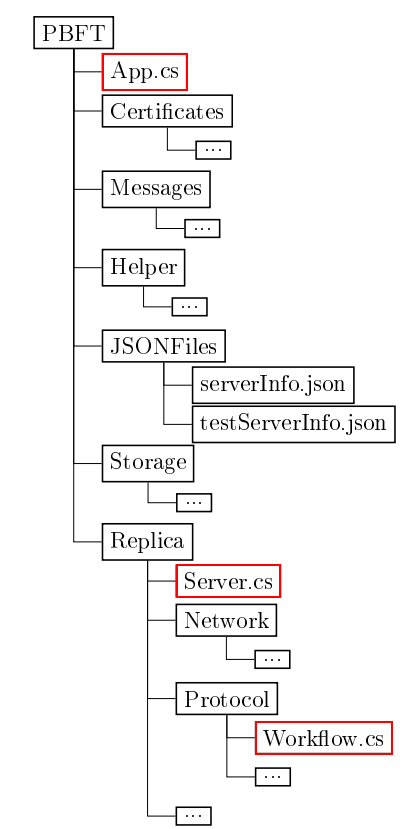
\includegraphics[width=0.45\linewidth]{figures/filestructtest}
	\caption{Summary of the file architecture for the PBFT implementation}
    \label{fig:filestruct}
\end{figure}

\newpage

\section{Persistent vs Ephemeral}
%This will be a very large part, just need to figure out how to structure it.
%Before we can introduce the main PBFT implementation workflow, it is first important to introduce the relationship between the server side and the protocol workflow. 
\label{sec:persvsephe}
An important detail when using the Cleipnir framework is to have a general idea for which parts of the system are desired to be persistent. As mentioned in \autoref{section:PersistentProgramming}, Cleipnir allows for hybrid persistent programming. Therefore, it is important to know which data is needed to be persisted for the consensus algorithm, so that it can be easily reinstated after a system shutdown. In addition, it is important to avoid storing unnecessary data as it will generally slow down the synchronization period. Another reason as to why making a distinct divide between persistent and ephemeral parts of the code is important is due to the difficulties encountered when using \code{CTask} together with traditional asynchronous operations as mention in \autoref{section:PersistentProgramming}. In our case, because our goal is to evaluate both async/await and Cleipnir for implementation of consensus algorithms, its important to not interchange these tools as it would in most cases lead to race conditions.

\autoref{fig:PersistencyEphemeral} shows parts of our PBFT implementation being divided into persistent parts and ephemeral parts. In general, static functions and objects unrelated to the PBFT workflow are treated as ephemeral. Meanwhile objects related to the PBFT implementations, \code{Source} objects and functions that handles workflow related to the PBFT protocol are persisted. The server is an exception as some parts are persistent while others parts are not. As an example, the protocol logger is stored in the server and is persisted, on the other hand anything related to networking is not persisted. In a sense the operations occurring in the server are treated as a bridge between the persistent parts as well as the ephemeral parts. By this we mean the server is responsible for handling any messages received from the socket connections. These messages are then emitted to their respective reactive operators which are run in the persistent part and are waiting for changes to occur. There are a few exceptions to this rule, case in point if the message is needed for server-side rather than any PBFT protocol workflows, the message is instead used directly by the server. A primary example of this being session messages. However, in order for the servers non-persistent network handler to be perform operations which affects the persistent part run by Cleipnir, the operation must be scheduled by Cleipnir's execution engine. There are two reasons for this syntax. Firstly, code run by Cleipnir is not supposed to be affected by code outside of Cleipnir. Similarly to the case where using an asynchronous operations within \code{CTask}, attempting to emit a message or perform an operation which changes the state of a persisted object, will most of the time cause the same scenario we discussed earlier. New threads will occur and Cleipnir will attempt to perform the operation concurrently, however this scenario is not thread safe and sooner or later will affect the state of the system negatively. Secondly, running the operations by the Cleipnir's execution engine attempts to enforce the FCFS approach as mention in \autoref{section:CleipnirOv}. This will in turn make it a lot easier to keep track of the operations as it will give the illusion of synchronously system. The only situation we experienced where the Cleipnir execution engine didn't follow the FCFS scheduling algorithm was then the next operations was stuck, in which the second operation in the queue was executed instead and so forth. \autoref{code:schedulerEmit} shows an example of where the server uses the Cleipnir engine reference to schedule a phase message to be emitted to the \emph{ProtocolSubject} \code{Source} object. To summarize the primary relationship between the server, the network layer and the persistent workflow implementations is simply that the server will emit any messages it receives from the network layer and then emit these messages to the persistent workflows. As it is required for the PBFT protocol and view-change protocol to multicast messages during their process, these implementations have a direct reference to the server. In order to accomplish this, both persistent workflow shares a common persistent object known as \code{ProtocolExecution}. This means the protocol algorithms can easily send any messages it needs to the server through the server referance in the \code{ProtocolExecution}. 

This design is unfortunately not perfect. Because the server requires to schedule the operations in order for protocol execution to move on with its execution. In some scenarios we've encountered where the scheduled process never finishes its execution. Normally this wouldn't be a problem, however in some cases it is quite a severe problem. Usually when scheduling an operation which requires emitting to a \code{source} object without any receivers, the operation obviously will never finish. Nevertheless, when the server attempts to schedule an additional operations afterwards, the operation is never scheduled, which in turn leads to the application being deadlocked. This situation seems to be similar to sending messages to a channel without any receivers in Golang\cite{WEB:golangChannels}, in spite of that this is an issue which rarely occur, but when it does it is detrimental to the system. Therefore, to counteract this issue, strict conditions are placed in the server to avoid sending messages to reactive subjects in the situations where there are no listeners. %may be too vague.

\begin{figure}[H]
	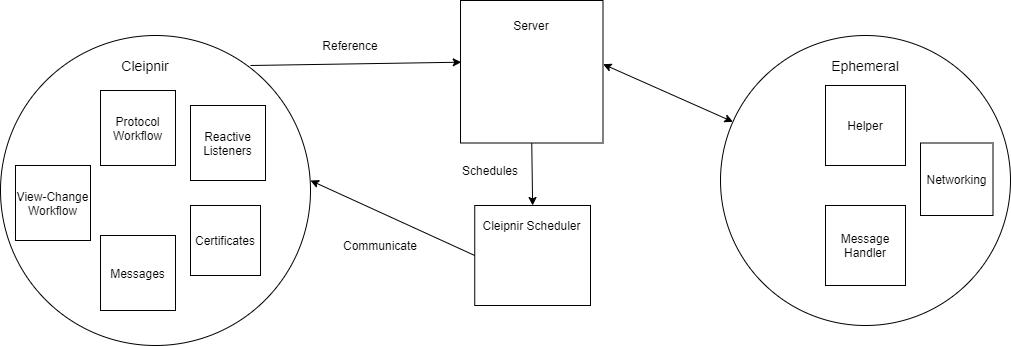
\includegraphics[width=\linewidth]{figures/CleipnirStructure}
	\caption{Application divided into persistent parts and ephermeral parts and how they interact}
	\label{fig:PersistencyEphemeral}
\end{figure}

\begin{figure}[h]
	\centering
	%\lstset{style=sharpc}
	\begin{lstlisting}[label = code:schedulerEmit, caption= Example of server and protocol interaction using Cleipnir scheduler, captionpos=b, basicstyle=\scriptsize]
	public void EmitPhaseMessageLocally(PhaseMessage mes)
        {
            Console.WriteLine("Emitting Phase Locally!");
            if (ProtocolActive)
            {
                _scheduler.Schedule(() =>
                {
                    Subjects.ProtocolSubject.Emit(mes);
                });    
            }
        }
	\end{lstlisting}
\end{figure}